\chapter{Experimental Apparatus}\label{ch:experiment}

\section{Large Hadron Collider}

The Large Hadron Collider (LHC)~\cite{Evans:2008zzb} is a superconducting synchrotron that accelerates two counter-rotating, circular beams of hadrons and collides them at four interaction points (IPs) where experiments are placed, as depicted in Fig.~\ref{lhc-overview}. It is operated by the European Organization for Nuclear Research (CERN), which is headquartered in Geneva, Switzerland, and is their flagship experiment. \correction{The LHC is installed in the 26.7~km circumference tunnel that was used by the CERN Large Electron-Positron collider and lies beneath the France-Switzerland border at depths as low as 175~m below the surface.} It accelerates separate beams of protons (p) or lead ions (Pb) yielding pp, pPb, or PbPb collisions. The LHC primarily operates using pp collisions. Operation for production physics began in 2010. In October 2017, xenon (Xe) beams were successfully tested and XeXe collisions were achieved. 

\begin{figure}[!htb]
	\centering
	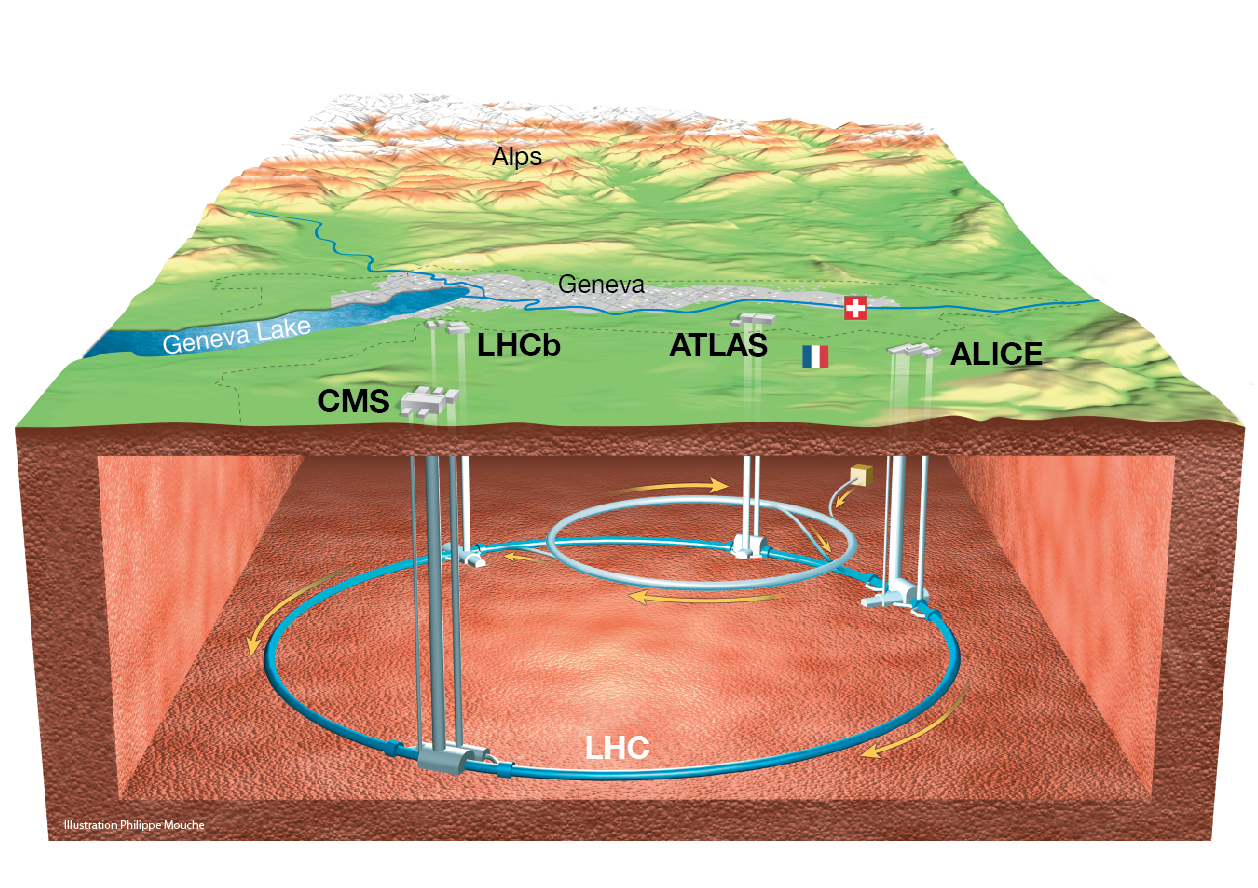
\includegraphics[scale=0.25]{figures/lhc_overview}
	\caption{An overview of the location of LHC and its four interaction points~\cite{Mouche:1708847}.}
	\label{lhc-overview}
\end{figure}

\subsection{The CERN Accelerator Complex}

The LHC is designed to achieve pp collisions at a center-of-mass energy $\sqrt{s} = 14\TeV$. Protons are delivered to the LHC after going through a series of stages in the CERN accelerator complex, as shown in Fig.~\ref{accelerator-complex}. During each stage, the proton's energy is steadily increased using older accelerators from the previous generations of CERN experiments.  

\begin{figure}[!htb]
	\centering
	\includegraphics[width=1.0\textwidth]{figures/CCC-v2018-print-v2.pdf}
	\caption{The CERN accelerator complex~\cite{Mobs:2636343}.}
	\label{accelerator-complex}
\end{figure}

Protons are sourced from a bottle of hydrogen gas which is ionized using electric fields. After ionization, the electrons are separated and the protons that are left behind are initially accelerated to 50\MeV using the Linac~2 linear accelerator. The beam is then sent to the circular Proton Synchrotron Booster where it reaches an energy of 1.4\GeV before being injected into the circular Proton Synchrotron and further accelerated to 25\GeV. Next, the beam is transferred to the nearly 7~km circumference Super Proton Synchrotron which accelerates the beam to an energy of 450\GeV. The protons are finally injected into the LHC where they reach their final center-of-mass energy of up to 14\TeV. After acceleration, the two counter-rotating beams are brought together and the protons are collided at the four IPs where detectors are placed.

\begin{figure}[!htb]
	\centering
	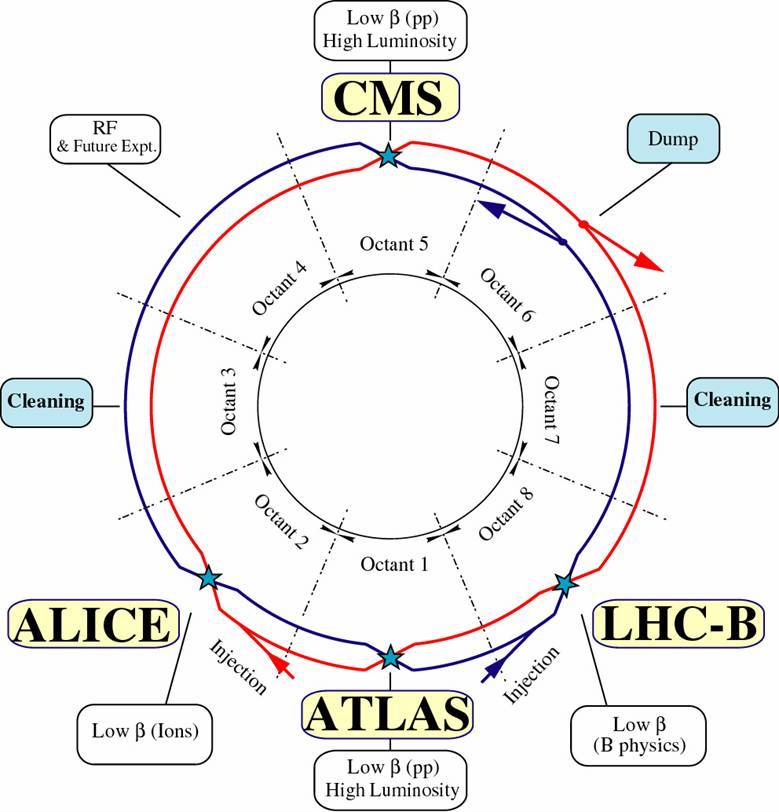
\includegraphics[scale=0.40]{figures/lhc-interaction-points}
	\caption{A schematic of the eight LHC insertion points~\cite{LHC_schematic}.}
	\label{lhc-ips}
\end{figure}

The LHC has insertions at its Points~1, 2, 5, and 8 housing the IPs where the respective ATLAS~\cite{Aad:2008zzm}, ALICE~\cite{Aamodt:2008zz}, CMS~\cite{Chatrchyan:2008aa}, and LHCb~\cite{Alves:2008zz} experiments are located. ATLAS and CMS are general purpose collider detectors designed to search for and study the Higgs boson, perform precision measurements of SM parameters, study strongly interacting matter, and search for evidence of physics beyond the SM. LHCb is designed to study heavy flavor physics, primarily searching for evidence of new physics in CP violation from beauty and charm hadron decays. ALICE is a general purpose heavy ion detector designed to study the physics of strongly interacting matter and the quark-gluon plasma. In addition to these four major LHC experiments, four more insertion points are used for LHC operations. Point 4 contains radio frequency (RF) cavities inserted to accelerate the particle beams. The insertions in Points~3 and 7 host collimators used for beam cleaning, and Point~6 contains the beam dump insertion. Fig.~\ref{lhc-ips} shows a schematic of the eight LHC insertion points, which includes the four IPs.


\subsection{The LHC Components}

The LHC uses RF cavities to accelerate the particle beams. Superconducting dipole electromagnets are used to bend the beams and quadrupole magnets are used for focusing. \correction{There are 1232 dipole and 392 quadrupole magnets around the LHC ring, each 15~m and 3~m long, respectively.} The dipole magnets are constructed using NbTi superconducting coils capable of generating an 8.3~T magnetic field. \correction{A cross-section of a dipole magnet is depicted in Fig.~\ref{lhc-dipole}.}

\begin{figure}[!htb]
	\centering
	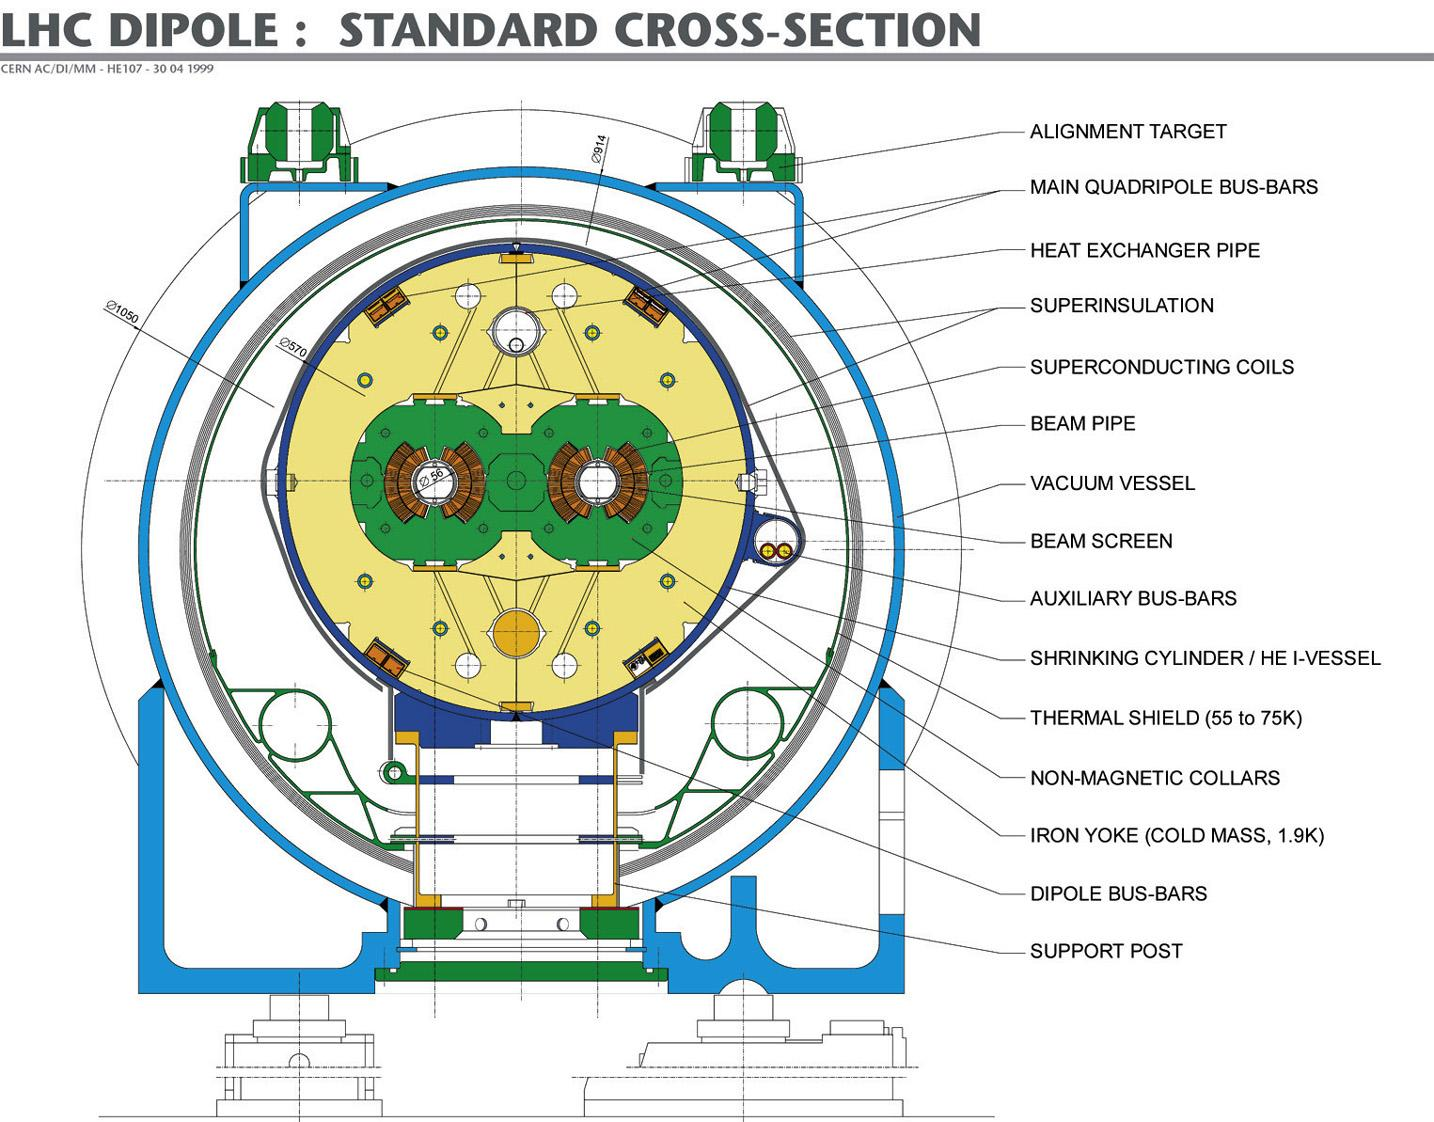
\includegraphics[scale=0.50]{figures/lhc_dipole}
	\caption{A cross-section of an LHC dipole magnet~\cite{Team:40524}.}
	\label{lhc-dipole}
\end{figure}

The proton beams are divided into bunches containing on the order of $10^{11}$~protons/bunch. At designed operation, bunches are spaced so that they occur 25~ns apart. Given the LHC orbit length of $89.1~\mu$s, a maximum of 3564 bunches are possible in each beam. Bunches are injected in the LHC in bunch trains separated by empty bunches which allow for beam monitoring, calibration, and control. At nominal operation, 2808 bunches are filled in each beam. The total number of events $N$ produced in the collisions are related to the integrated luminosity $L$ of the LHC fill by
\begin{equation}
	L = N\sigma
\end{equation}
where $\sigma$ is the proton-proton interaction cross section. The total proton-proton cross section at $\sqrt{s} = 14\TeV$ is expected to be roughly 100~mb~\cite{Bruning:782076}. At $\sqrt{s} = 13\TeV$, CMS measured the inelastic portion of this cross section to be approximately 70~mb in a restricted phase space of the detector~\cite{Sirunyan:2018nqx}. The integrated luminosity is calculated from the instantaneous luminosity $\mathcal{L}$ by the anticipated relation $L = \int \mathcal{L} \, \text{d}t$. The instantaneous luminosity is determined from the beam parameters by
\begin{equation}
	\mathcal{L} = \frac{N_{\mathrm{b}}^2 f n_{\mathrm{b}}}{4\pi\sigma_{\mathrm{x}}^*\sigma_{\mathrm{y}}^*}F
\end{equation}
where $N_{\mathrm{b}}$ is the number of protons/bunch, or beam intensity; $n_{\mathrm{b}}$ is the number of bunches; $f = 11.2455$~kHz is the LHC revolution frequency; $\sigma_{\mathrm{x,y}}^*$ are the transverse RMS beam widths at the IP; and $F$ is a geometric loss factor used to correct for the beam crossing angle, shape, and longitudinal beam size. For a Gaussian beam at nominal LHC operation, both $\sigma_{\mathrm{x}}^*$ and $\sigma_{\mathrm{y}}^*$ equal $16.6~\mu$m. The loss factor is about 0.83~\cite{Bruning:782076}. The instantaneous luminosity is not constant throughout the period of duration during stable beam collisions. This is primarily due to beam intensity degradation and emittance growth. The luminosity decays with a lifetime $\tau$ according to
\begin{equation}
	\mathcal{L} = \mathcal{L}_0e^{-t/\tau}
\end{equation}
where $\mathcal{L}_0$ is the peak instantaneous luminosity, which, at nominal pp LHC operation, is on the order of $10^{34} \;\text{cm}^{\texttt{-}2} \, \text{s}^{\texttt{-}1}$. A snapshot of the LHC status display, taken during pp collisions, is given in Fig.~\ref{fig:lhc_fill_decay}, showing the decay in instantaneous luminosity over time as measured by the LHC experiments. The lifetime during stable beam collisions is about 20~hours. However, during typical operation, stable beams can be lost to electrical trips or contamination in the beam pipe.

\begin{figure}[!htb]
	\centering
	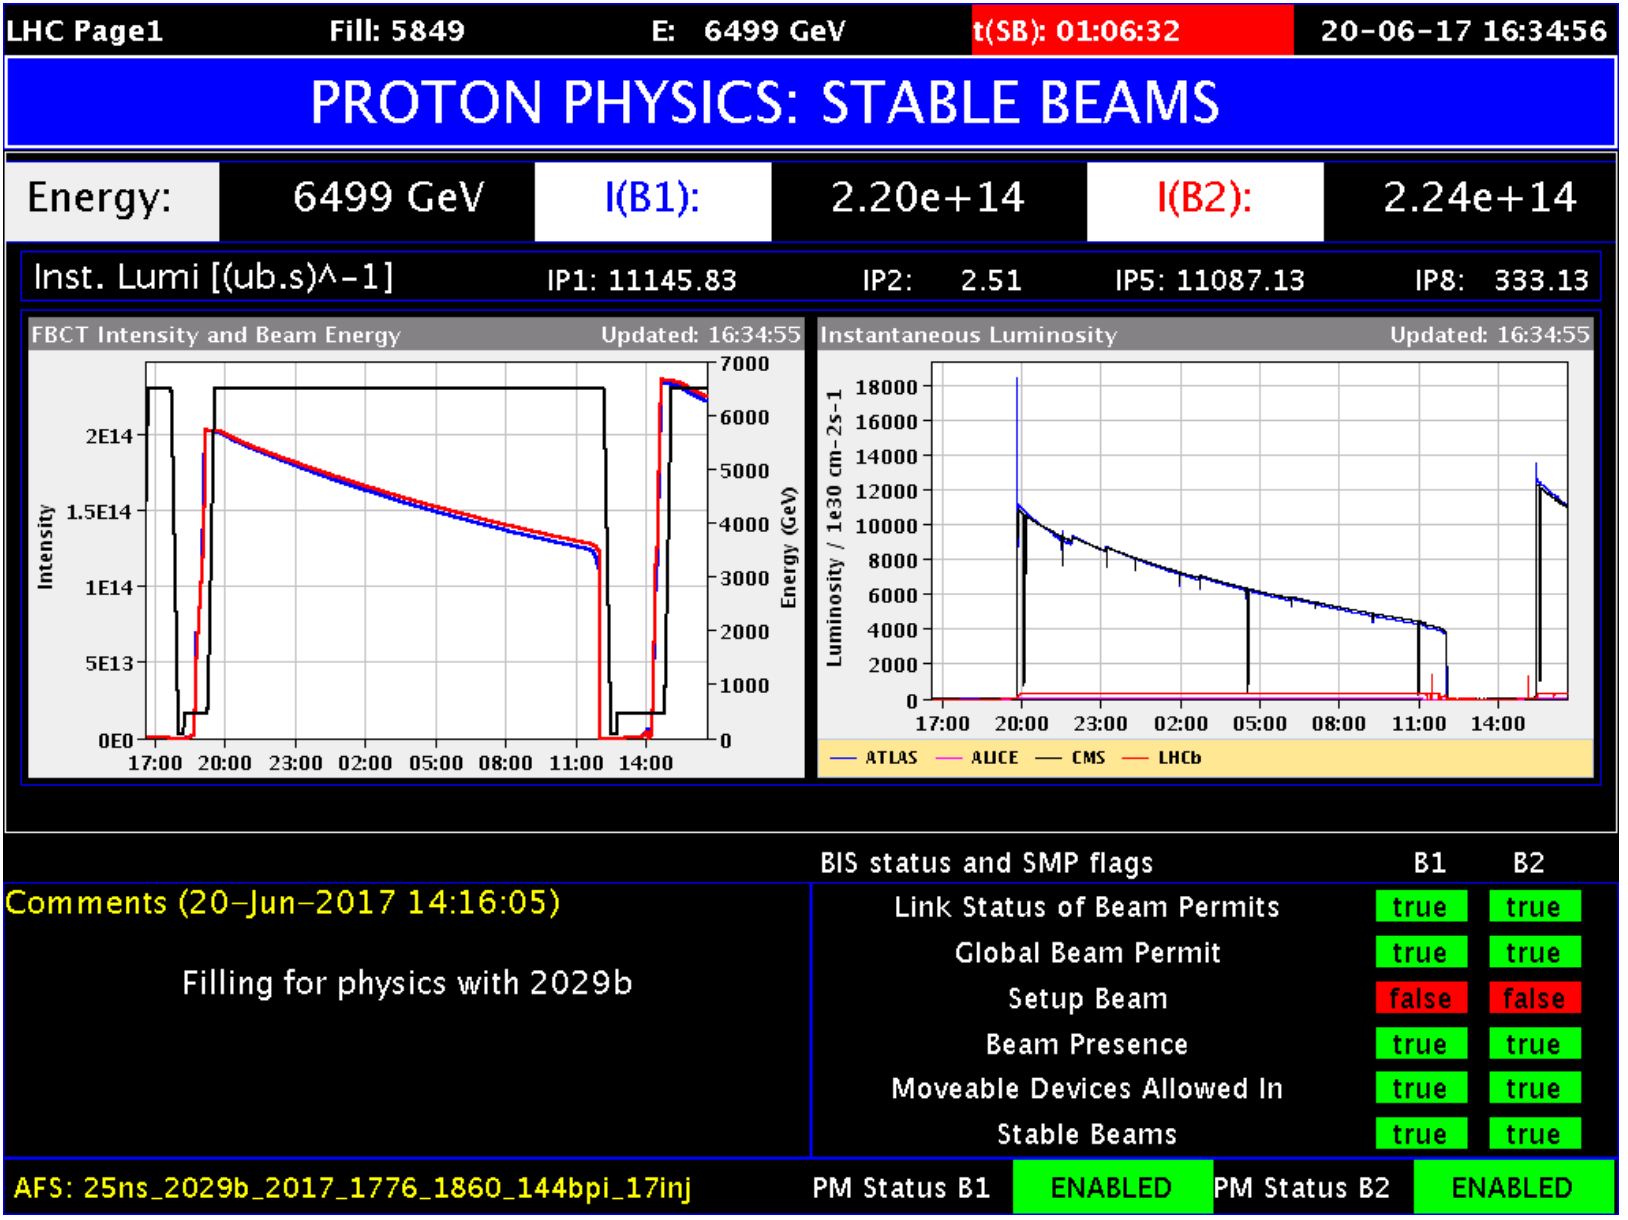
\includegraphics[width=0.80\textwidth]{figures/lhc_fill_decay}
	\caption{A snapshot of the LHC status display, taken in June 2017 during stable beam pp physics collisions, showing the decay in instantaneous luminosity over time as measured by the LHC experiments.}
	\label{fig:lhc_fill_decay}
\end{figure}


\subsection{The LHC Schedule}

The LHC operates during production cycles known as Runs, which typically last for 3-4~years. During any year within an LHC running period, stable proton-proton collisions used for production physics are only performed for part of that year. For the other part of that year, the LHC is shutdown for about 3-4~months to accommodate upgrades and repairs and additional running time is allocated for beam commissioning, special requests by the experiments for beam use, and heavy ion collisions. Runs are followed by an extended period of accelerator inactivity without beams known as a Long Shutdown (LS). During this time, major upgrades and repairs are performed on the accelerator and each of its experiments. The first pp collisions were achieved in November 2009 and physics production began in March 2010, marking the start of the Run~1 LHC physics program. The current planned longterm LHC schedule is summarized in Table~\ref{tab:LHC_schedule}.

\begin{table}[htbp!]
	\caption{A summary of the current planned longterm LHC schedule. A tentative schedule extends past LS3.}
	\label{tab:LHC_schedule}
	\centering
  \vspace{\baselineskip}
	\begin{tabular}{ll}
	\hline \hline
	LHC period & Duration \\
	\hline
	Run 1 & 2010-2012 \\
	LS1   & 2013-2014 \\
	Run 2 & 2015-2018 \\
	LS2   & 2019-2020 \\
	Run 3 & 2021-2023 \\
	LS3   & 2024- \\
	\hline \hline
	\end{tabular}
\end{table}

During the first part of Run~1 from 2010-2011, the LHC performed pp collisions at $\sqrt{s} = 7\TeV$. In 2010, the LHC delivered an integrated luminosity of 44.9\pbinv, of which 41.5\pbinv were recorded by CMS. In 2011, this increased to 6.1\fbinv being delivered and 5.6\fbinv recorded. The collision energy for pp collisions was increased to $\sqrt{s} = 8\TeV$ during the second part of Run~1 beginning in 2012. This resulted in the LHC providing an integrated luminosity of 23.3\fbinv, of which CMS recorded 21.8\fbinv and certified 19.7\fbinv for physics analysis use. During Run~1, a 50~ns bunch spacing was used.

Starting with Run~2, the collision energy was further increased to $\sqrt{s} = 13\TeV$. During the first two months of physics data taking, a 50~ns bunch spacing was used, but, in August 2015, this spacing was reduced to the nominal LHC value of 25~ns, where it remains. In 2015, the LHC delivered 4.2\fbinv with 3.8\fbinv of it recorded by CMS. This increased as the LHC delivered an integrated luminosity of 40.8\fbinv to CMS in 2016 and 49.8\fbinv in 2017, of which 37.8\fbinv and 45\fbinv was recorded, respectively. \correction{In 2018, 68.2\fbinv were delivered by the LHC and 64\fbinv were recorded by the CMS detector, using the current best offline data reconstruction. Future improvements in the offline reconstruction could change the final numbers. This marks the end of Run~2. In total, 163\fbinv were delivered by the LHC and 150.5\fbinv were recorded by CMS with 139.7\fbinv being certified for physics analysis use in Run~2. During Runs~1 and~2, a combined integrated luminosity of approximately 192.5\fbinv were delivered by the LHC to the CMS detector.} A summary of this during each year of Runs~1 and~2 is shown in Fig.~\ref{fig:lumi_cms}. Also shown is a detailed breakdown for 2016, which is the year the dataset used by the analysis in this dissertation was recorded. For more information on the CMS luminosity measurement in 2016, see Ref.~\cite{CMS-PAS-LUM-17-001}.

A major goal during LS2 is to prepare the LHC for reaching its nominal collision energy of $\sqrt{s} = 14\TeV$, planned for Run~3 operation. By the end of Run~3, it is expected that many of the LHC components will suffer severe radiation damage and will need to be replaced. Therefore, at the start of LS3, the LHC is planned to be upgraded to the High-Luminosity Large Hadron Collider (HL-LHC)~\cite{Apollinari:2284929}. The HL-LHC is being designed to integrate ten times more luminosity than the LHC. This high luminosity environment poses significant challenges to the LHC experiments and will require them to undergo major changes, especially in the forward region of the detectors. To accommodate this, the CMS Collaboration, in particular, is preparing for its Phase II upgrade~\cite{Contardo:2020886,Butler:2055167}, which includes a proposal to replace its existing endcap calorimeters with a high granularity calorimeter~\cite{Collaboration:2293646}. 

\begin{figure}[!htbp]
	\centering
	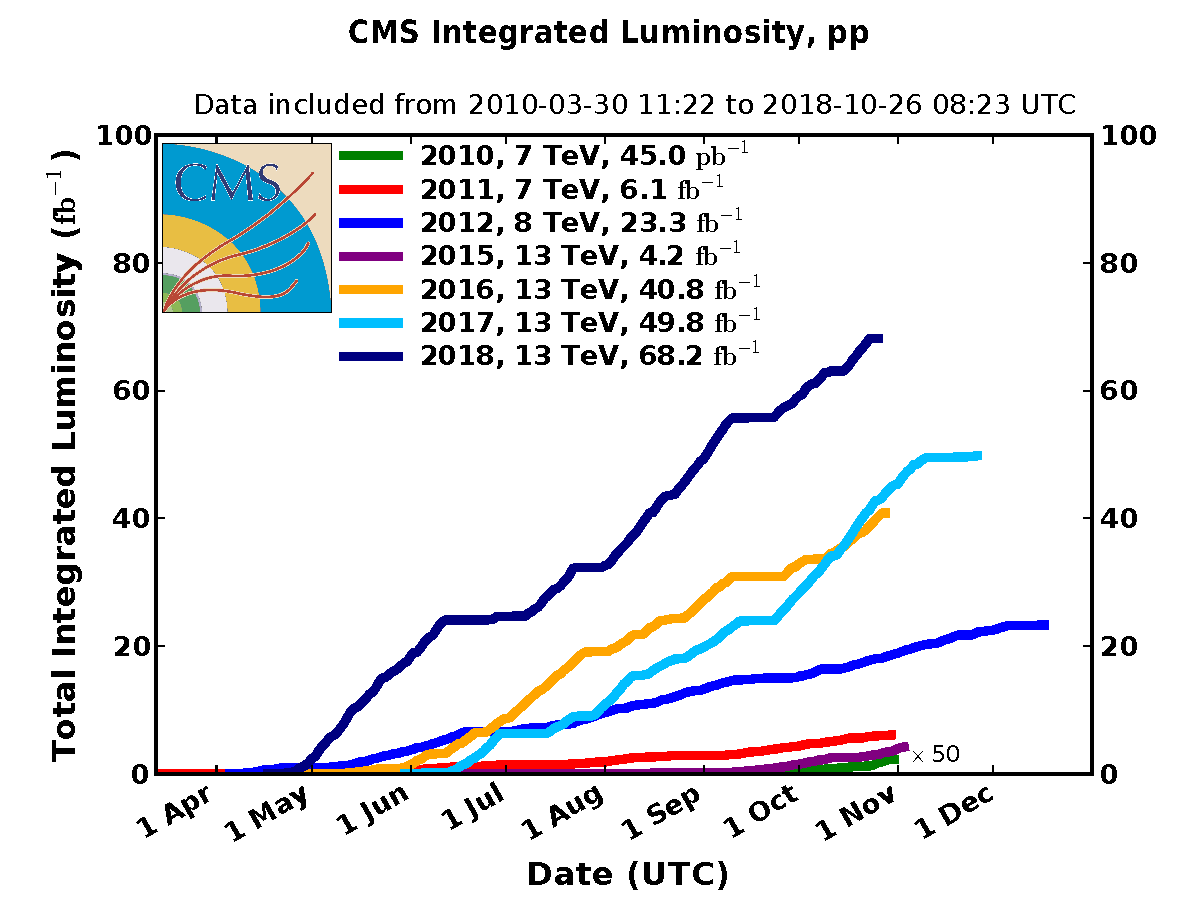
\includegraphics[scale=0.40]{figures/int_lumi_cumulative_pp_2.pdf}
	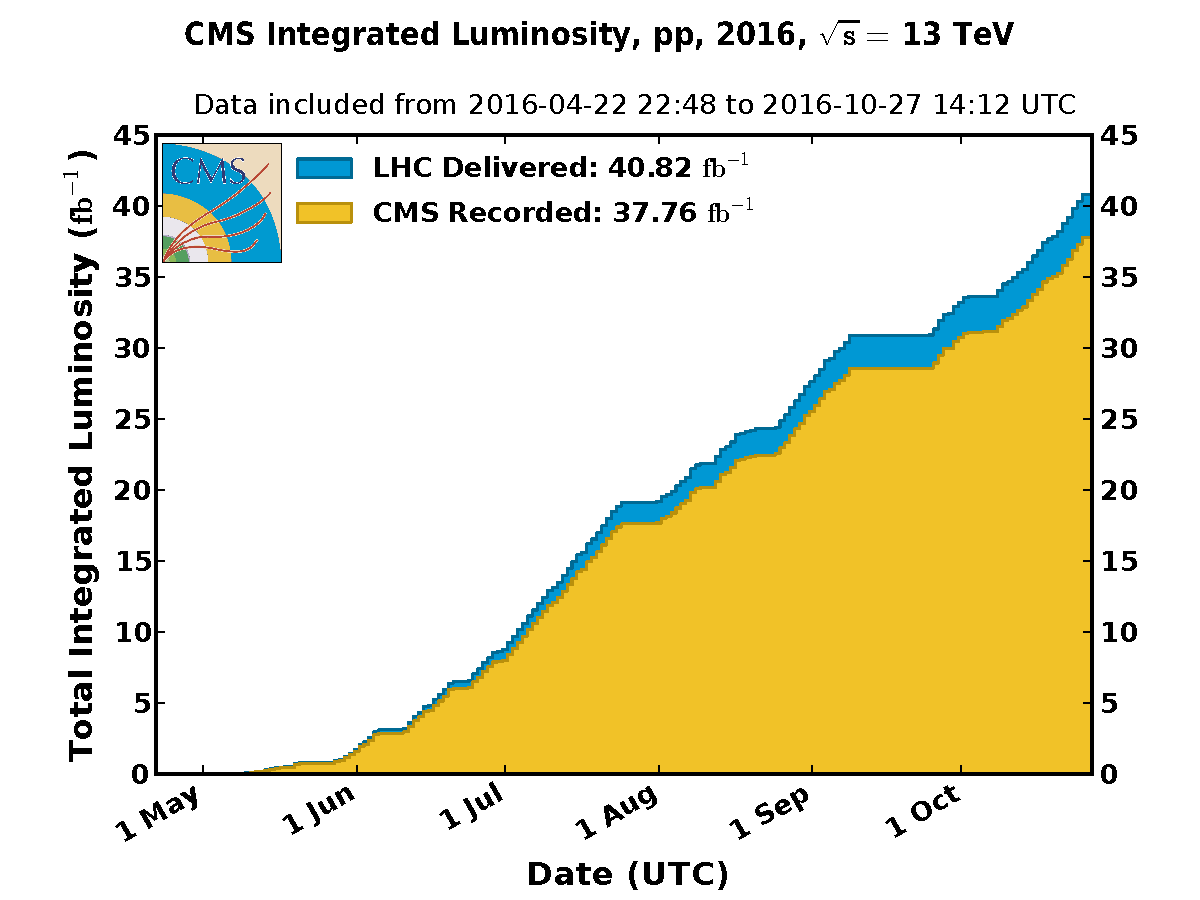
\includegraphics[scale=0.40]{figures/int_lumi_per_day_cumulative_pp_2016.pdf}
	\caption{A timeline showing the cumulative (left) and detailed 2016 (right) integrated luminosity delivered by the LHC~\cite{CMS_lumi}. The amount recorded by CMS in 2016 is also shown.}
	\label{fig:lumi_cms}
\end{figure}


\section{The CMS Detector}

The Compact Muon Solenoid (CMS) detector~\cite{Chatrchyan:2008aa} is a general purpose particle physics experiment designed for high performance in the search for the Higgs boson and for BSM physics at the {\TeVns} scale. It operates as one of the LHC experiments located underground at Point~5 of the LHC ring located in Cessy, France. The overall detector has a cylindrical form approximately 15~m in diameter and 28.7~m in length, weighing about \correction{14000 metric tons}. A defining feature of CMS is its 6~m internal diameter superconducting solenoid, providing a uniform magnetic field of 3.8~T inside the majority of its detector volume. CMS comprises several subdetectors arranged in a barrel and endcap configuration, centered on the beam axis, consisting of an inner silicon pixel and strip tracking system; a crystal electromagnetic calorimeter (ECAL); a brass and scintillator hadron calorimeter (HCAL), all of which are mostly contained inside of the solenoid; and gas ionization muon chambers embedded in the steel return yoke of the solenoid. Fig.~\ref{CMS} depicts a 3D cutaway model of the CMS detector, highlighting its major components in this configuration.

\begin{figure}[!htb]
	\centering
	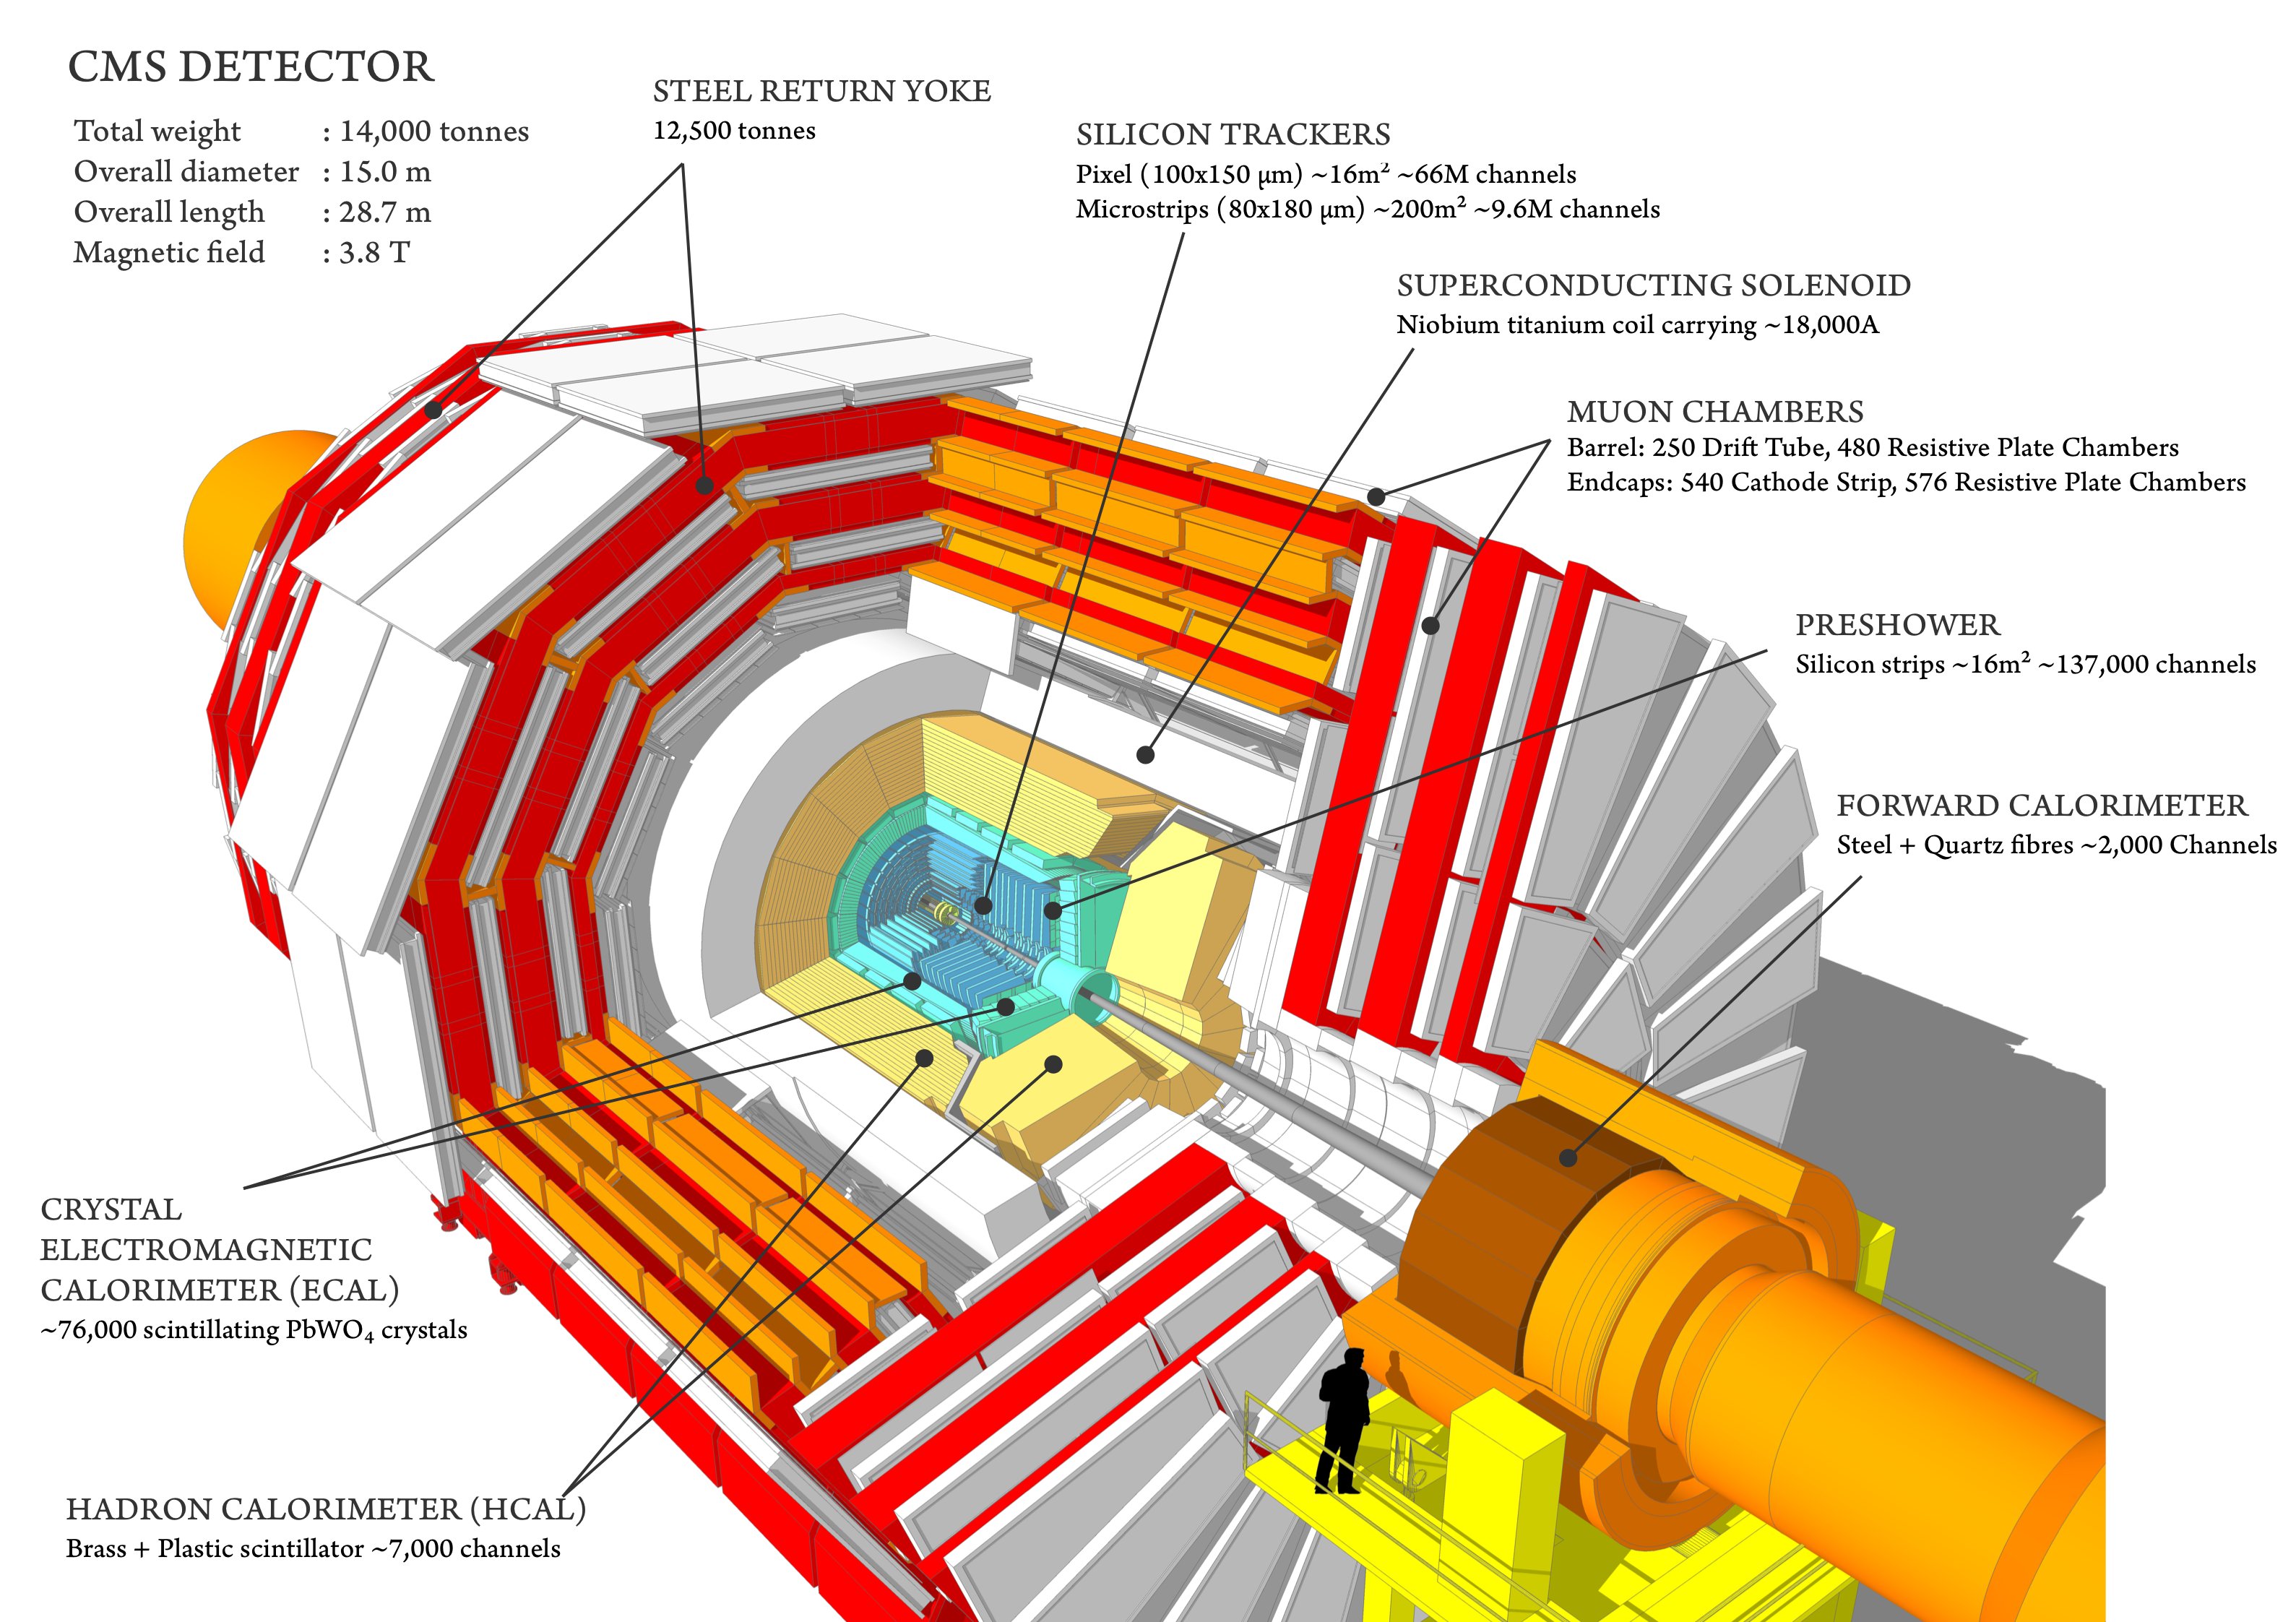
\includegraphics[width=1.0\textwidth]{figures/cms_sketchup}
	\caption{An overview of the CMS detector and its major components~\cite{Sakuma:2013jqa}.}
	\label{CMS}
\end{figure}

Particle detection in CMS relies on information from each subdetector, starting with the inner most detectors. Different particles interact differently with the various detector technologies, possibly leaving behind tracks or energy deposits in different regions, as depicted in Fig.~\ref{cms-slice}. This information is read out using a sophisticated trigger and data acquisition system, consisting of the detector electronics, Level-1 trigger, readout network, and high-level trigger. After describing the CMS coordinate system, we will discuss each of its major components.

\begin{figure}[!htbp]
	\centering
	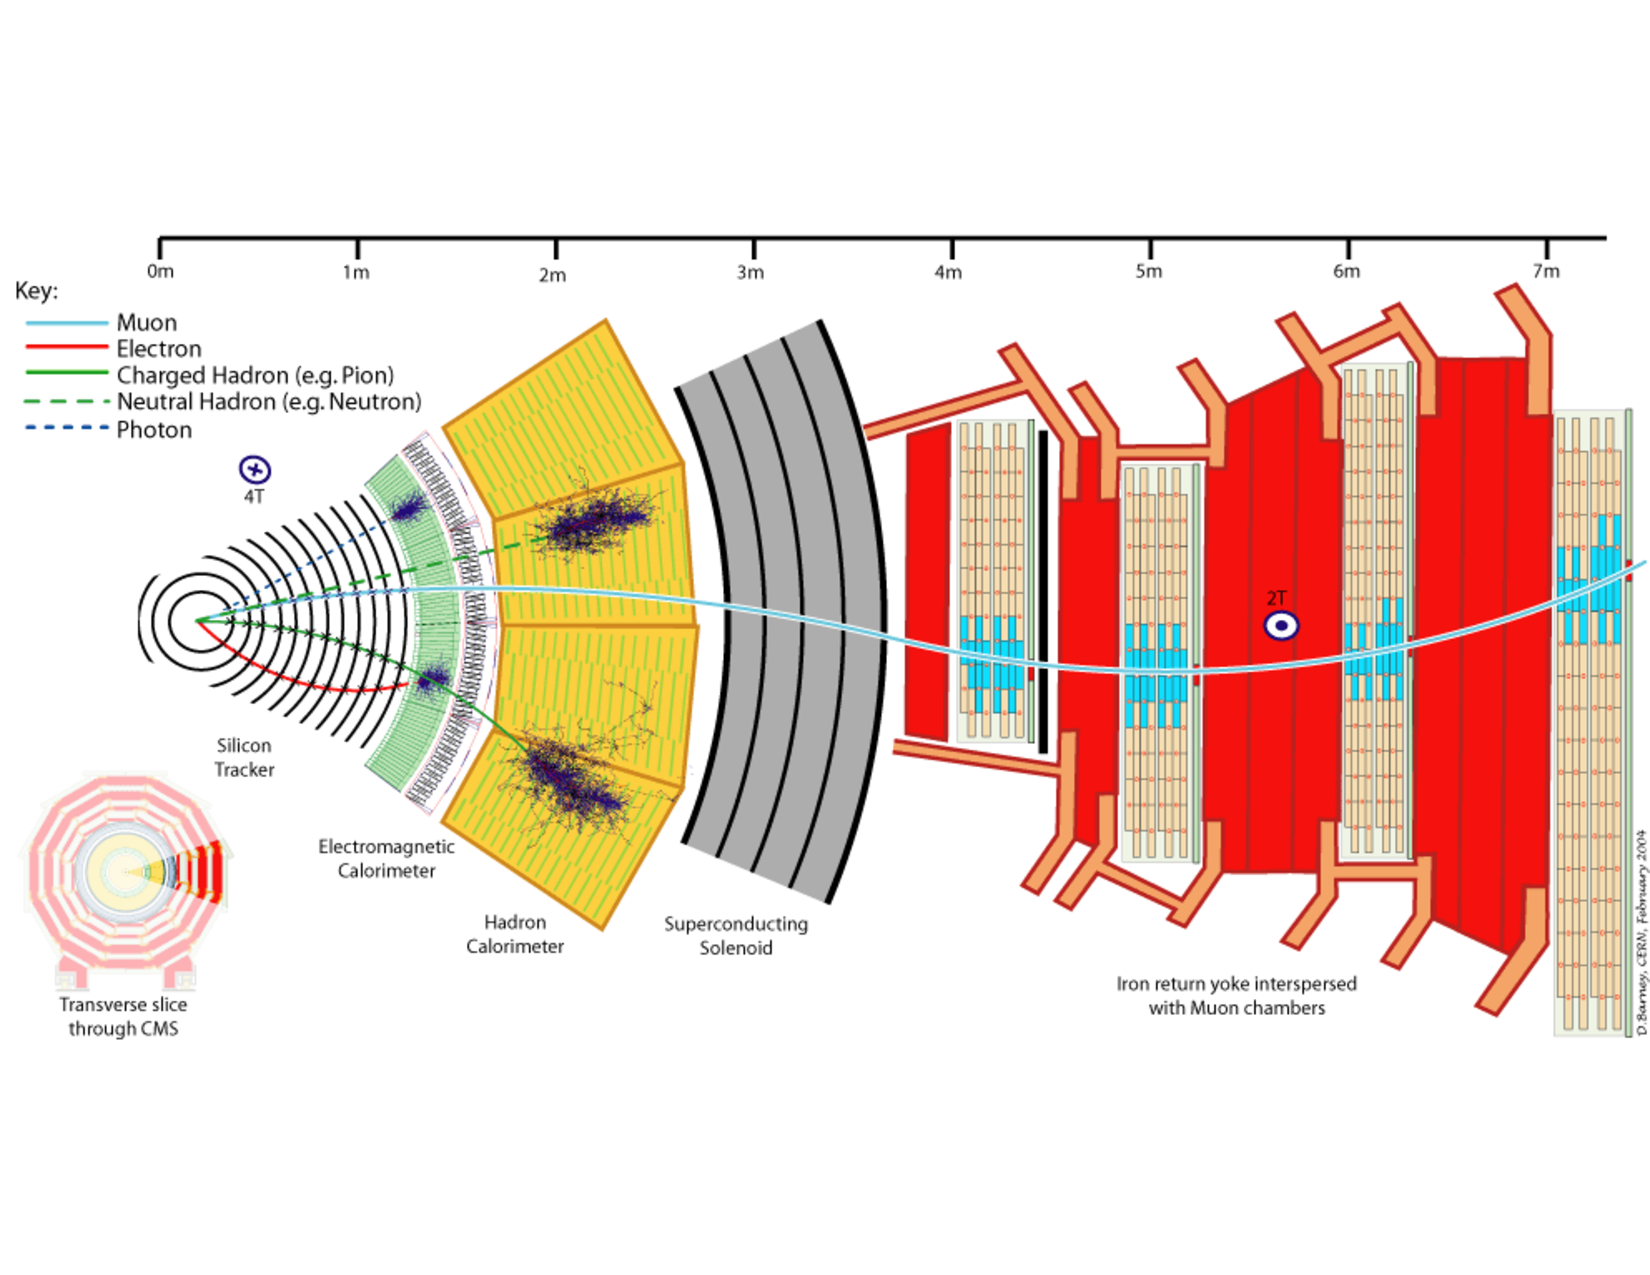
\includegraphics[width=1.0\textwidth]{figures/CMS_slice.pdf}
	\caption{A transverse slice of the CMS detector highlighting how different particles interact with its various detector technologies~\cite{Davis:2205172}.}
	\label{cms-slice}
\end{figure}


\subsection{Coordinate System}

CMS uses a right-handed coordinate system with its origin located at the nominal LHC interaction point inside of the detector. The $x$-axis points inward towards the center of the LHC, the $y$-axis points vertically upward perpendicular to the LHC plane, and the $z$-axis points along the direction of the counterclockwise rotating beam. Due to its geometry, cylindrical coordinates of the form $(z,\theta,\phi)$ are used. The azimuthal angle $\phi$ is measured from the $x$-axis in the transverse $x$-$y$ plane, and the polar angle $\theta$ is measured from the $z$-axis. A diagram illustrating both the Cartesian and cylindrical coordinate systems is shown in Fig.~\ref{fig:coordinate_system}. 

\begin{figure}[!htb]
	\centering
	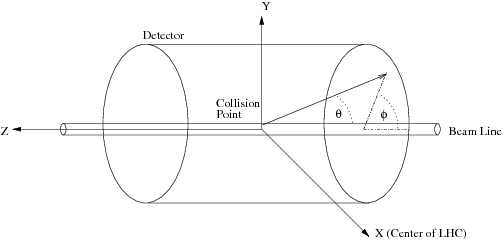
\includegraphics[scale=0.75]{figures/coordinate_system.png}
	\caption{An illustration of the coordinate system used by the CMS detector~\cite{Schott:1699952}.}
	\label{fig:coordinate_system}
\end{figure}

Measurements of particle energy $E$ and momentum $p$ in the transverse plane are denoted $E_{\mathrm{T}} = E \sin\theta$ and $\pt = p \sin\theta$, respectively. Typically, the pseudorapidity, defined as $\eta = - \ln[\tan(\theta/2)]$, is preferred to $\theta$. Particle coordinates are often expressed as $(\pt, \eta, \phi)$, with distances in the $\eta$-$\phi$ plane given by $\Delta R = \sqrt{(\Delta\phi)^2 + (\Delta\eta)^2}$.


\subsection{Inner Tracking System}

The inner tracking system of CMS is designed to measure the trajectories of charged particles emerging from the collisions, as well as perform the reconstruction of secondary vertices, such as from $b$ quark and $\tau$ lepton decays. This system consists of the silicon pixel and strip tracker subdetectors, laid out according to Fig.~\ref{fig:tracker}.

\begin{figure}[!htb]
	\centering
	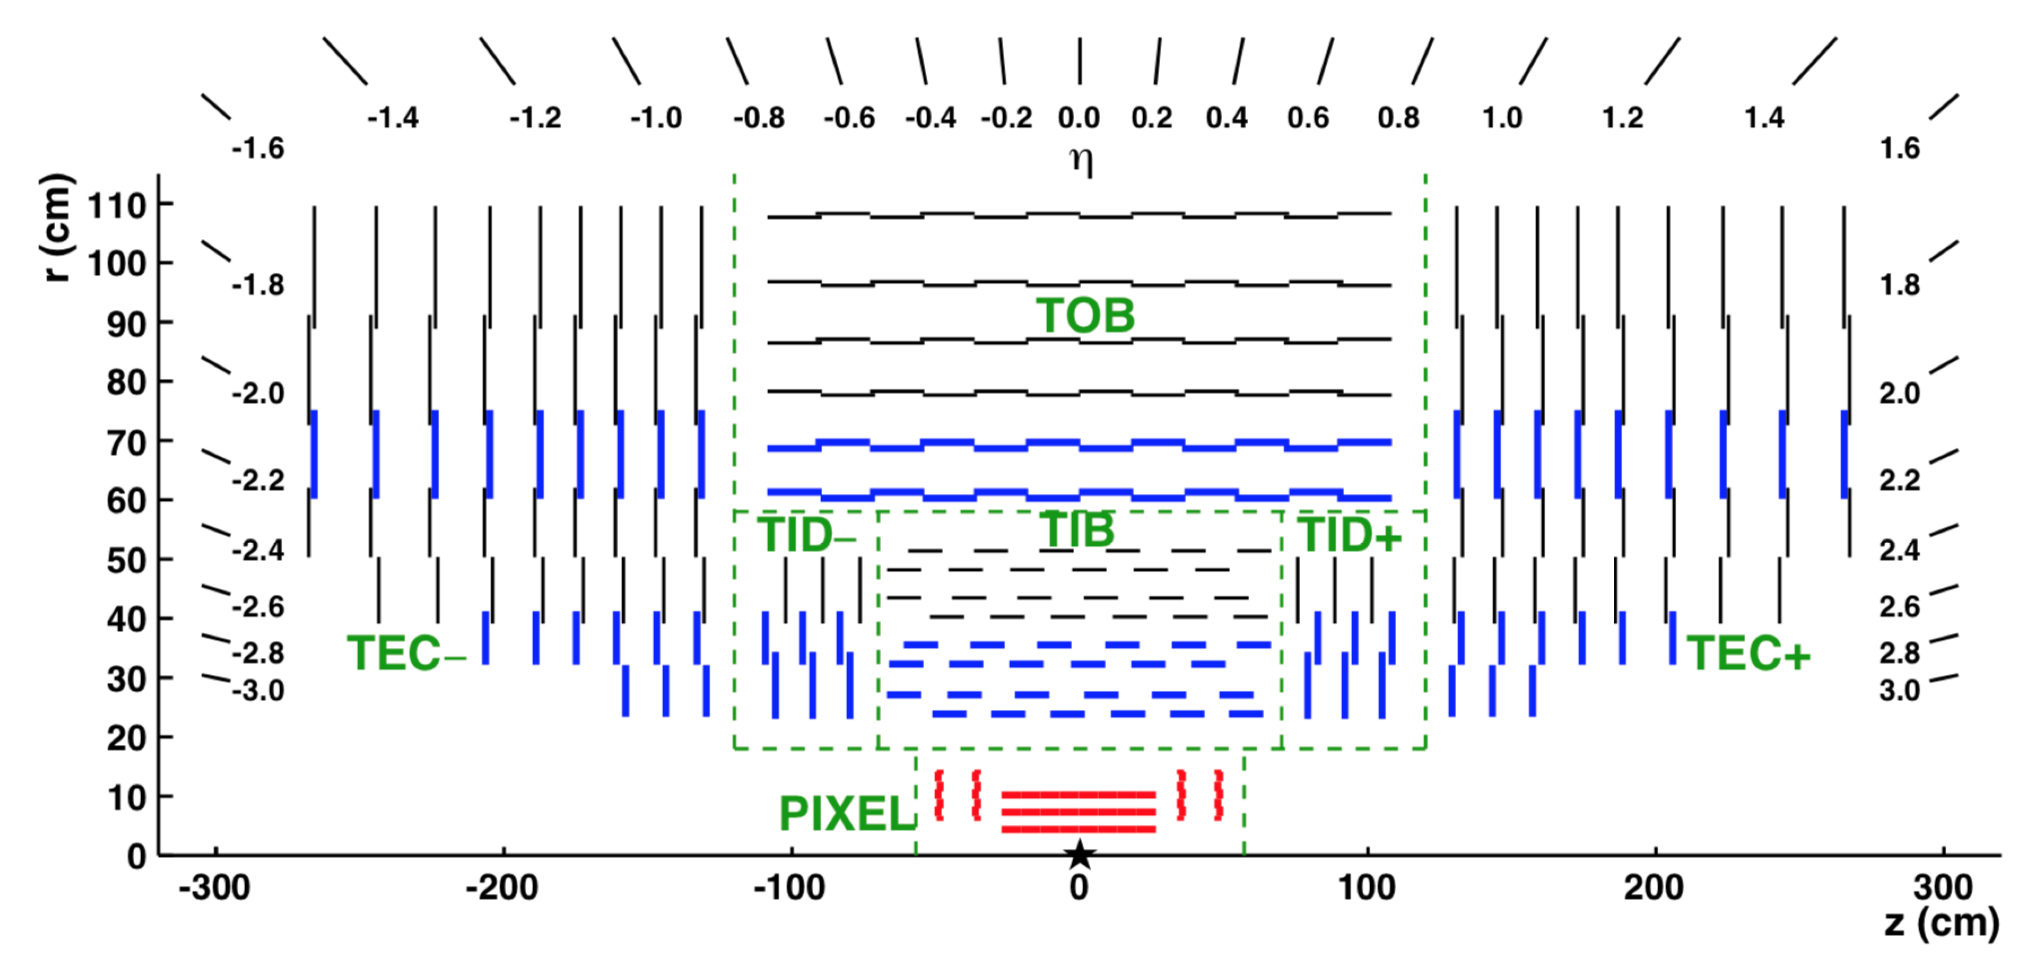
\includegraphics[width=0.85\textwidth]{figures/inner_tracker.png}
	\caption{A schematic of the CMS inner tracking system~\cite{Sirunyan:2018icq}.}
	\label{fig:tracker}
\end{figure}

The silicon pixel detector consists of 3 barrel layers (BPix) and 2 endcap disks (FPix), which surround the interaction point, providing coverage in the range $-2.5<\eta<2.5$. The BPix layers are 53~cm long and located at radii of 4.4, 7.3, and 10.2~cm. The FPix are placed at $z=\pm34.5$ and $\pm46.5$~cm with radii ranging from 6-15~cm. A single silicon pixel cell has an area of $100{\times}150$~$\mu$m. In total, the BPix (FPix) consists of 48 (18) million pixels covering an area of 0.78 (0.28)~$\textrm{m}^2$.

The silicon strip tracker consists of four subsystems: the tracker inner barrel (TIB), tracker inner disks (TIDs), tracker outer barrel (TOB), and tracker endcaps (TECs). Both the TIB and TIDs are located out to $r=55$~cm and comprise 320~$\mu$m thick silicon microstrip sensors arranged in 4 barrel layers and 3 disks, respectively. This inner barrel and disk system is surrounded by the TOB, which has an outer radius of 116~cm and extends between $z=\pm118$~cm. The TOB consists of 6 barrel layers of 500~$\mu$m thick silicon microstrip sensors. The TECs cover the range $124<|z|<282$~cm, surrounding the rest of the system. Each TEC comprises 9 disks with radii ranging between 22.5-113.5~cm, using silicon strips either 320 or 500~$\mu$m thick. The entire strip tracker has a total of 9.3 million silicon strips covering a total area of 198~$\textrm{m}^2$.

The performance of the inner tracking system is presented in Ref.~\cite{Chatrchyan:2014fea}, and the reconstruction of tracks and vertices is discussed in Section~\ref{sec:event_reco}.


\subsection{Electromagnetic Calorimeter}\label{sec:ECAL}

The electromagnetic calorimeter (ECAL) is designed to detect and measure the energy of electrons and photons. The ECAL is a hermetic, homogeneous calorimeter comprising approximately 75000 lead tungstate (PbW$\text{O}_4$) scintillating crystals separated into a barrel (EB) and two endcap (EE) sections, which give coverage up to $|\eta|<3.0$. These crystals were chosen for their high granularity, short radiation length, high radiation tolerance, and fast response time. Avalanche photodiodes are used to detect the scintillation light in the EB and vacuum phototriodes are used in the EEs. The scintillation light is caused by high-energy electrons or photons initiating an electromagnetic shower in the crystals. This occurs for electrons when they undergo bremsstrahlung until their energy loss becomes dominated by ionization and for photons when they undergo pair production until their energies fall below the pair production threshold. The electromagnetic shower ionizes the atoms in the crystals and light is emitted when they de-excite. The amount of light produced is proportional to the energy of the incident particles. A general description of the passage of particles through matter and, in particular, their detection using calorimeters is given in Sections~33 and~34 of Ref.~\cite{Tanabashi:2018oca}.

The EB is located at $y = 1.29$~m and covers the range $|\eta| < 1.479$. It is made up of 61200 crystals constructed into 36 identical supermodules, each covering half of the barrel length. Each supermodule is made up of 4 modules, and these modules are made up of various submodules each containing 2 rows of 5 crystals. The gap between adjacent crystals is 320~$\mu$m. A single crystal in the EB covers an area of about $22{\times}22$~m$\text{m}^2$ in $\eta$-$\phi$, giving a granularity of $\Delta\eta{\times}\Delta\phi = 0.0174{\times}0.0174$. Each crystal is of length 230~mm, corresponding to 25.8 radiation lengths ($X_0$). The crystals are tilted at $3^{\circ}$ with respect to the origin in both the $\eta$ and $\phi$ directions, allowing for the detection of particles that would otherwise travel between the gaps of the crystals.


Each EE is located at $z = \pm 3.14$~m and covers the range $1.479 < |\eta| < 3.0$. They are made up of a total of 14648 crystals. Both are divided into two half-disk arrangements constructed with crystals tapered in an $x$-$y$ grid, grouped into $5{\times}5$ structures called supercrystals. A single crystal in an EE covers an area of about $28.6{\times}28.6$~m$\text{m}^2$ in $x$-$y$ and is of length 220~mm, corresponding to 24.7~$X_0$. The gap between adjacent crystals is 320~$\mu$m and between different $5{\times}5$ units is 2~mm.

A preshower detector (ES) is placed in front of each EE in the region $1.653 < |\eta| < 2.6$. These are primarily used to help distinguish between photons and $\pi^0$ decays which mimic a single photon signature. The ES is a sampling calorimeter made of 2 disks of lead and 2 planes of silicon strip detectors, providing about 3~$X_0$ of material. A cutaway view of the ECAL highlighting its main features is shown in Fig.~\ref{ecal}.

\begin{figure}[!htb]
	\centering
	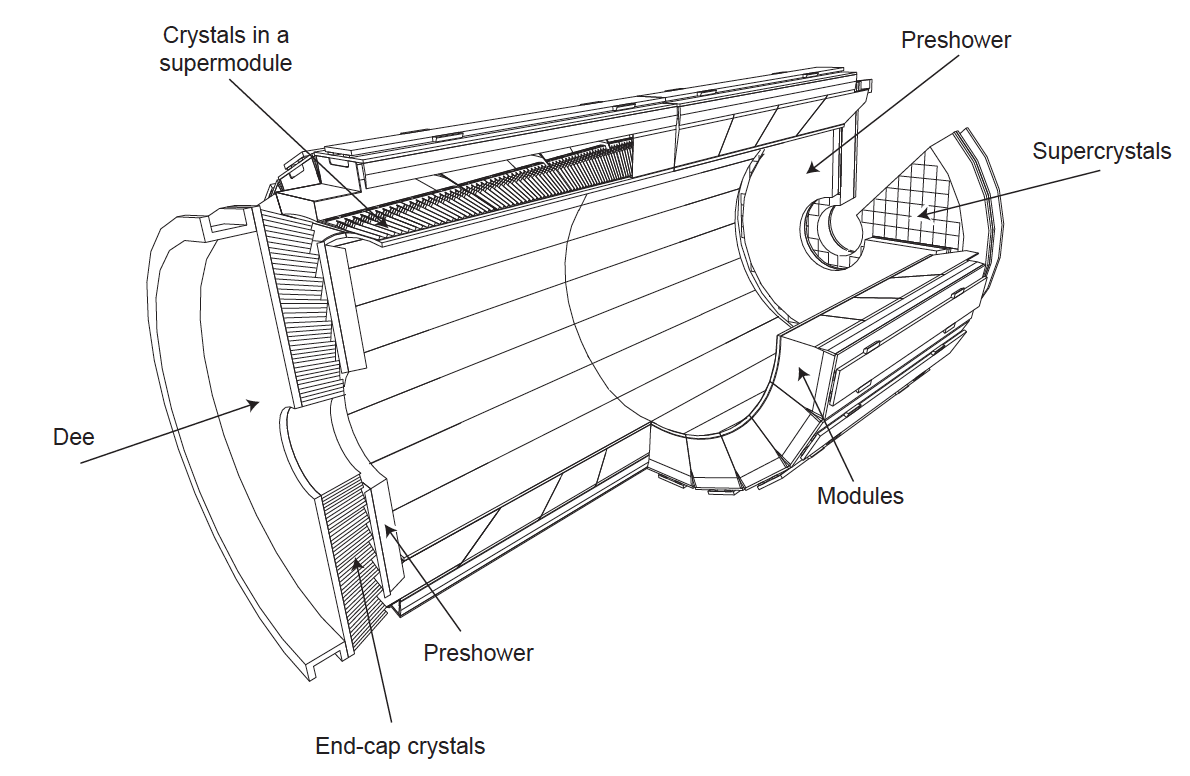
\includegraphics[scale=0.55]{figures/ecal}
	\caption{A cutaway view of the ECAL depicting its main features~\cite{Chatrchyan:2008aa}.}
	\label{ecal}
\end{figure}

The ECAL uses an active laser monitoring system to measure the relative response of laser light injected into the crystals. \correction{The response degrades over time as high radiation doses are received, with limited recovery during periods without collisions, as shown in Fig.~\ref{ecal_laser}.} These measurements are performed every 40 minutes and are used to correct the physics data. 

\begin{figure}[!htb]
	\centering
	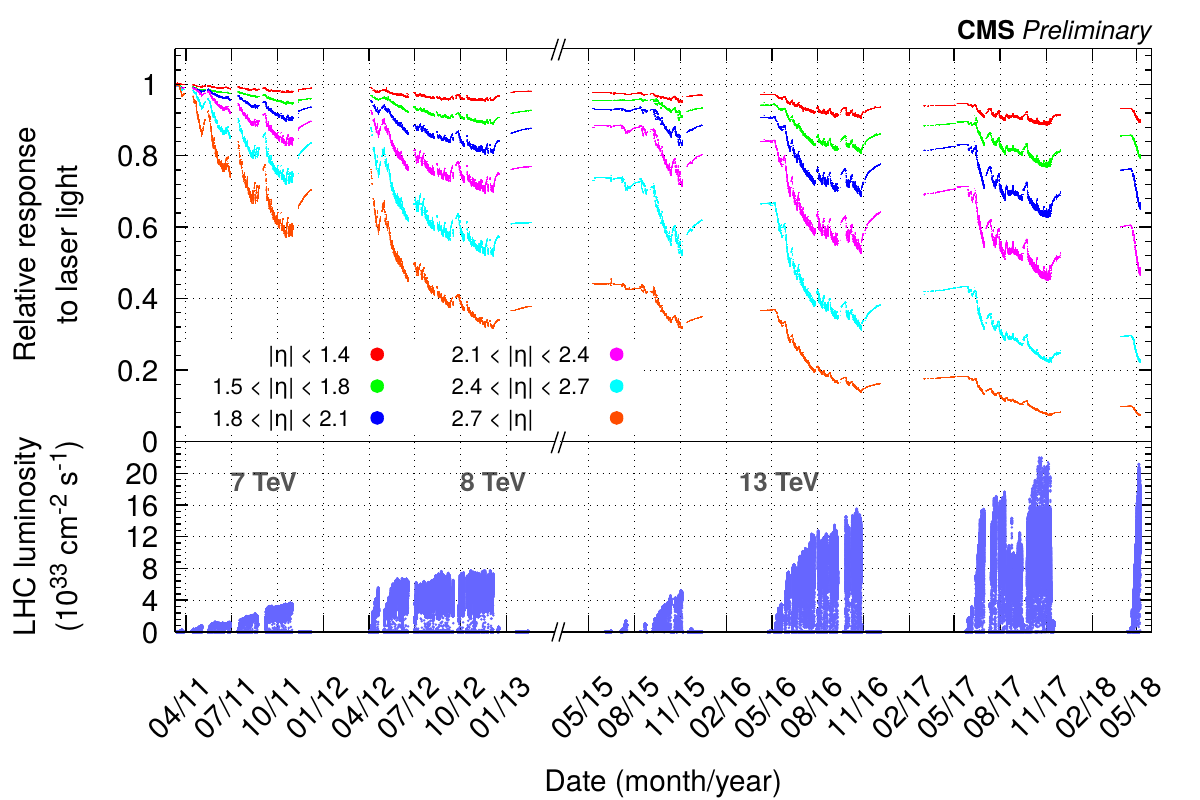
\includegraphics[width=0.85\textwidth]{figures/ecal_laser}
	\caption{The ECAL crystal response measured by the ECAL laser monitoring system over the LHC data taking periods~\cite{CMS-DP-2018-015}.}
	\label{ecal_laser}
\end{figure}

The energy resolution of the ECAL as a function of energy $E$ is characterized by separate terms added in quadrature of the form
\begin{equation}
	\frac{\sigma_E}{E} = \frac{a}{\sqrt{E}}\,\oplus\,\frac{b}{E}\,\oplus\,c
\end{equation}
for a stochastic term $a$, a noise term $b$, and a constant term $c$. The stochastic term arises from the statistical nature of the shower containment and is primarily caused by intrinsic shower fluctuations and photoelectron statistics. The noise term is primarily due to electronic noise, and the constant term is largely dependent on the intercalibration of the readout channels among different crystals. At high energies, the constant term dominates, but is corrected for and reduced by the laser monitoring system. All of these parameters were measured using an electron test beam and were determined to be $a = 2.8\%$, $b = 12\%$, and $c = 0.3\%$~\cite{Chatrchyan:2013dga}. The ECAL provides an energy resolution of about 2\% in the EB and about 2-5\% in the EE~\cite{Chatrchyan:2013dga}, as measured using $Z \to e^+e^-$ decays. A detailed description of the energy resolution measurement can be found in Ref.~\cite{CMS:EGM-14-001} for photons and Ref.~\cite{Khachatryan:2015hwa} for electrons. The reconstruction of electrons and photons is discussed in Section~\ref{sec:event_reco}.


\subsection{Hadron Calorimeter}

The hadron calorimeter (HCAL) is a hermetically constructed sampling calorimeter used to detect and measure the energy of hadronic particles. This is achieved by using alternating layers of absorber and scintillator materials. In most of the HCAL, brass is used as the absorber and plastic scintillator tiles are used as the sampling material. As a hadron travels through the HCAL, it interacts with the absorber, causing a hadron shower. This shower produces scintillation light in the tiles, which is carried through wavelength-shifting fibers to photodetectors. The photodetectors collect and convert the light pulses into electrical signals. The sum of the light across the entire shower is proportional to the energy of the incident hadrons.

The HCAL comprises four subdetectors: the hadron barrel (HB), hadron endcap (HE), hadron outer (HO), and hadron forward (HF) detectors. Fig.~\ref{hcal} shows a 2D projection of a quarter of the CMS detector, highlighting the $\eta$ coverage of each HCAL subdetector.

\begin{figure}[!htb]
	\centering
	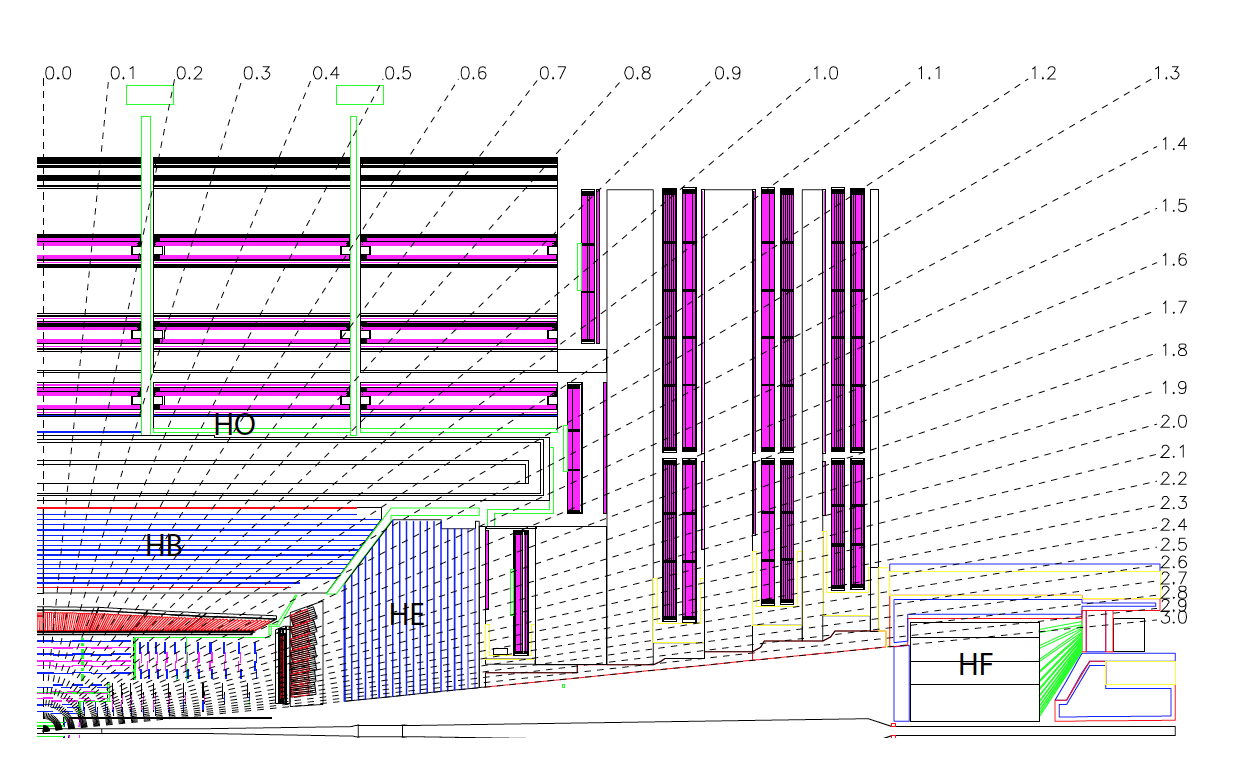
\includegraphics[scale=0.65]{figures/hcal}
	\caption{A projection of the HCAL, highlighting its subdetectors~\cite{Chatrchyan:2008aa}.}
	\label{hcal}
\end{figure}

The HB comprises 36 identical wedges forming two cylindrical half-barrels, each 4.3~m long. This subdetector extends radially between $1.77 < r < 2.95$~m and is located between the EB and solenoid, covering the region $|\eta| < 1.3$. Although the HB provides excellent shower containment in this region, the HO is added outside of the solenoid, which it uses as an absorber, to provide additional detection for shower tails that may extend outside of the HB. The combination of the HB and HO provide an effective thickness of a minimum of 11.8 nuclear interaction lengths ($\lambda_\mathrm{I}$). Each HE is located between $3.9 < |z| < 5.7$~m  and covers the range $1.3 < |\eta| < 3.0$. The granularity provided by the HB and HEs is $\Delta\eta{\times}\Delta\phi = 0.087{\times}0.087$ for $|\eta| < 1.6$ and $\Delta\eta{\times}\Delta\phi = 0.174{\times}0.174$ for $|\eta| \ge 1.6$. The scintillation light from the tiles across the depth of a single $\Delta\eta{\times}\Delta\phi$ region in the HB or an HE is optically added, forming a tower.

The coverage provided by the HEs is extended by the HFs to $|\eta| = 5.2$. Each HF is located at $z = 11.2$~m and uses quartz fibers embedded in a steel absorber to deal with some of the highest particle fluxes in the detector, minimizing radiation damage. Particle showers in the fibers emit Cherenkov radiation, which is detected by photomultiplier tubes. Each HF uses both long and short fibers interlaced throughout its detector volume. Both fibers run the full HF depth of 165~cm (10~$\lambda_\mathrm{I}$), but the short fibers start 22~cm from the front end. Both fibers are read out separately to allow for the discrimination between electromagnetic and hadron showers. The former deposit most of their energy within the first 22~cm, while the latter produce nearly equal signals in both calorimeter segments.


\subsection{Muon System}

The muon system is designed to provide robust muon identification with precise measurements of muon momenta. This subdetector is arranged in a muon barrel (MB) and muon endcap (ME) configuration, consisting of three types of gas ionization chambers: drift tube chambers (DTs), cathode strip chambers (CSCs), and resistive plate chambers (RPCs). The DTs are segmented into drift cells that measure the positions of muons by determining a drift time through an electric field to an anode wire of a cell. The CSCs are multi-wire proportional counters using a highly segmented cathode strip readout capable of providing an accurate measurement of the positions of the muons in the $r$-$\phi$ magnetic bending plane. The RPCs are double-gap chambers that operate in avalanche mode with a fast response and primarily provide timing information for the muon trigger. These chambers are embedded in the steel flux-return yoke outside of the solenoid. Fig.~\ref{fig:muon_system} shows a schematic highlighting these different features of the muon system.

\begin{figure}[!htb]
	\centering
	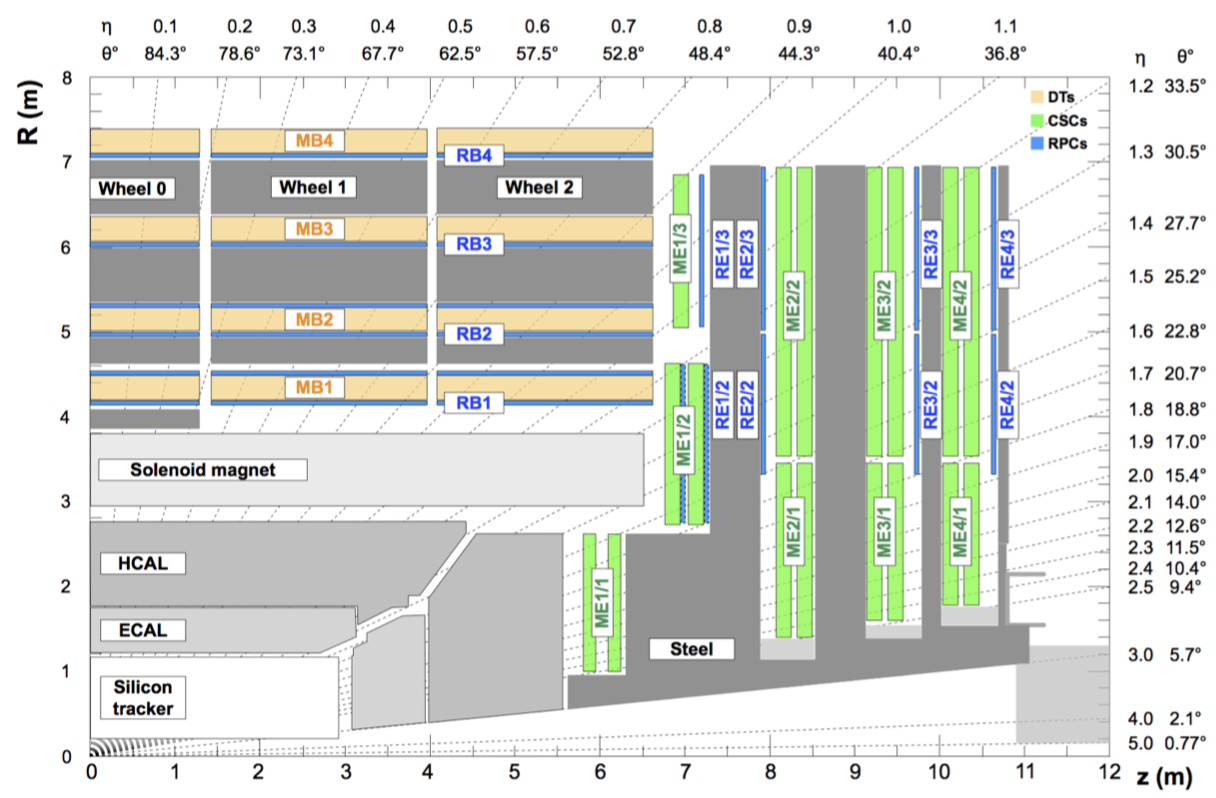
\includegraphics[width=0.85\textwidth]{figures/muon_chambers.png}
	\caption{A schematic of the CMS muon system depicting its major components and their detector coverage~\cite{Sirunyan:2018fpa}.}
	\label{fig:muon_system}
\end{figure}

The MB covers the region with $|\eta| < 1.2$ using DTs, chosen for the suitable detector conditions in that region: a uniform magnetic field, low neutron induced background, and small muon rates. The DTs are arranged into 4 stations, containing 8 chambers capable of measuring the muon position in the $r$-$\phi$ plane. The first 3 stations have 4 additional chambers allowing for position measurements along the $z$-axis. The MEs cover the region between $0.9 < |\eta| < 2.4$ using CSCs, which can handle the non-uniform magnetic field, high background levels, and large muon rates. Each ME has 4 stations of CSCs comprised of chambers positioned perpendicular to the beam line, providing the full position measurements and beam crossing times for the muons. To complement the DTs and CSCs, the RPCs are added to both the MB and MEs, covering $|\eta| < 1.6$. Their fast response provides good time resolution, but, compared to the DTs and CSCs, a coarser position resolution. There are 6 layers of RPCs embedded in the MB and 3 layers in each ME. Altogether, this provides a muon system capable of triggering on muon \pt with high efficiency ($>$90\% over the entire $\eta$ range) and excellent background rejection, while providing a muon \pt resolution of less than 7\% in the MB for muon $\pt < 1\TeV$ and a muon timing resolution of approximately 1.4~ns~\cite{Sirunyan:2018fpa}. The performance of the muon system is presented in Ref.~\cite{Sirunyan:2018fpa}, and further discussion on muon reconstruction is given in Section~\ref{sec:event_reco}.


\subsection{Trigger System}

The LHC provides proton-proton collisions at high rates, occurring every 25~ns, corresponding to a frequency of 40~MHz. This challenging environment is further complicated by the presence of pileup, which is multiple pp interactions occurring within the same event from a single proton-proton bunch crossing. This type of pileup is in-time with the bunch crossing, but pileup can also occur out-of-time from bunch crossings just before and after the collision of interest. When a subdetector's electronics are integrated for more than 25~ns, its response becomes sensitive to out-of-time pileup. The amount of pileup recorded by the CMS detector during each of its data taking years is plotted in Fig.~\ref{fig:CMS_pileup}. \correction{An average of 37 simultaneous pp interactions occurred during the 2018 LHC data taking period} using $\sqrt{s} = 13\TeV$. At these high rates with this large amount of pileup, it is not feasible to fully process, reconstruct, and store all of the data for each event, so a significant reduction needs to be made. This is accomplished by the trigger system, which functions in two stages: the Level-1 (L1) trigger and high-level trigger (HLT) stages.

\begin{figure}[!htb]
	\centering
	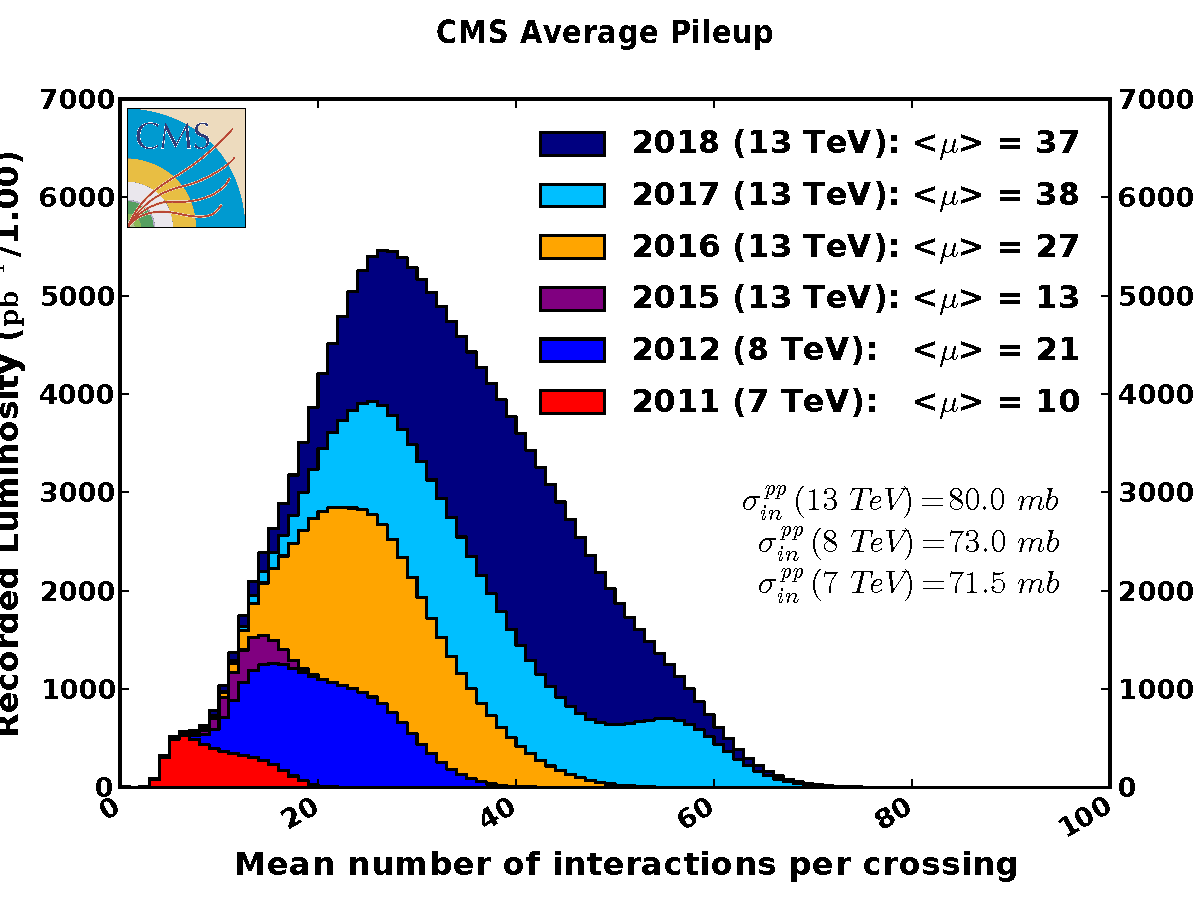
\includegraphics[width=0.63\textwidth]{figures/pileup_allYears_stack.pdf}
	\caption{The average amount of pileup recorded by the CMS detector during each of its data taking years~\cite{CMS_lumi}. The histograms from each year are stacked on the previous year. Also printed are the measured pp interaction cross sections for the different center-of-mass energies used during each data taking period.}
	\label{fig:CMS_pileup}
\end{figure}

The L1 trigger is made up of custom designed and programmable hardware. It analyzes every bunch crossing and is capable of selecting events in order to determine whether or not they should be further processed. This is achieved at a rate of around 100~kHz, with a latency of 3.2~$\mu$s. The L1 trigger uses information from the ECAL, HCAL, and muon system. The inner tracking system takes too long for readout at this stage and is only read out after the event of interest passes the L1 trigger. The calorimeters provide the L1 trigger with trigger primitives based on the presence of large energy deposits. This information is passed to regional and global components of the trigger, where event-level quantities are determined, such as jets, photon/electron candidates, traverse energy, and missing transverse energy. The muon system works to provide track information and muon candidates. The L1 trigger takes the final information provided by these subsystems and generates an L1 Accept (L1A) if trigger criteria are met, marking the event to be fully read out. Upon generation of an L1A, the detector information is passed to the HLT, which reconstructs the event and decides whether or not it should be saved. These steps are described in the flowchart in Fig.~\ref{fig:L1_trigger}. A more detailed description can be found in Ref.~\cite{Khachatryan:2016bia}.

\begin{figure}[!htb]
	\centering
	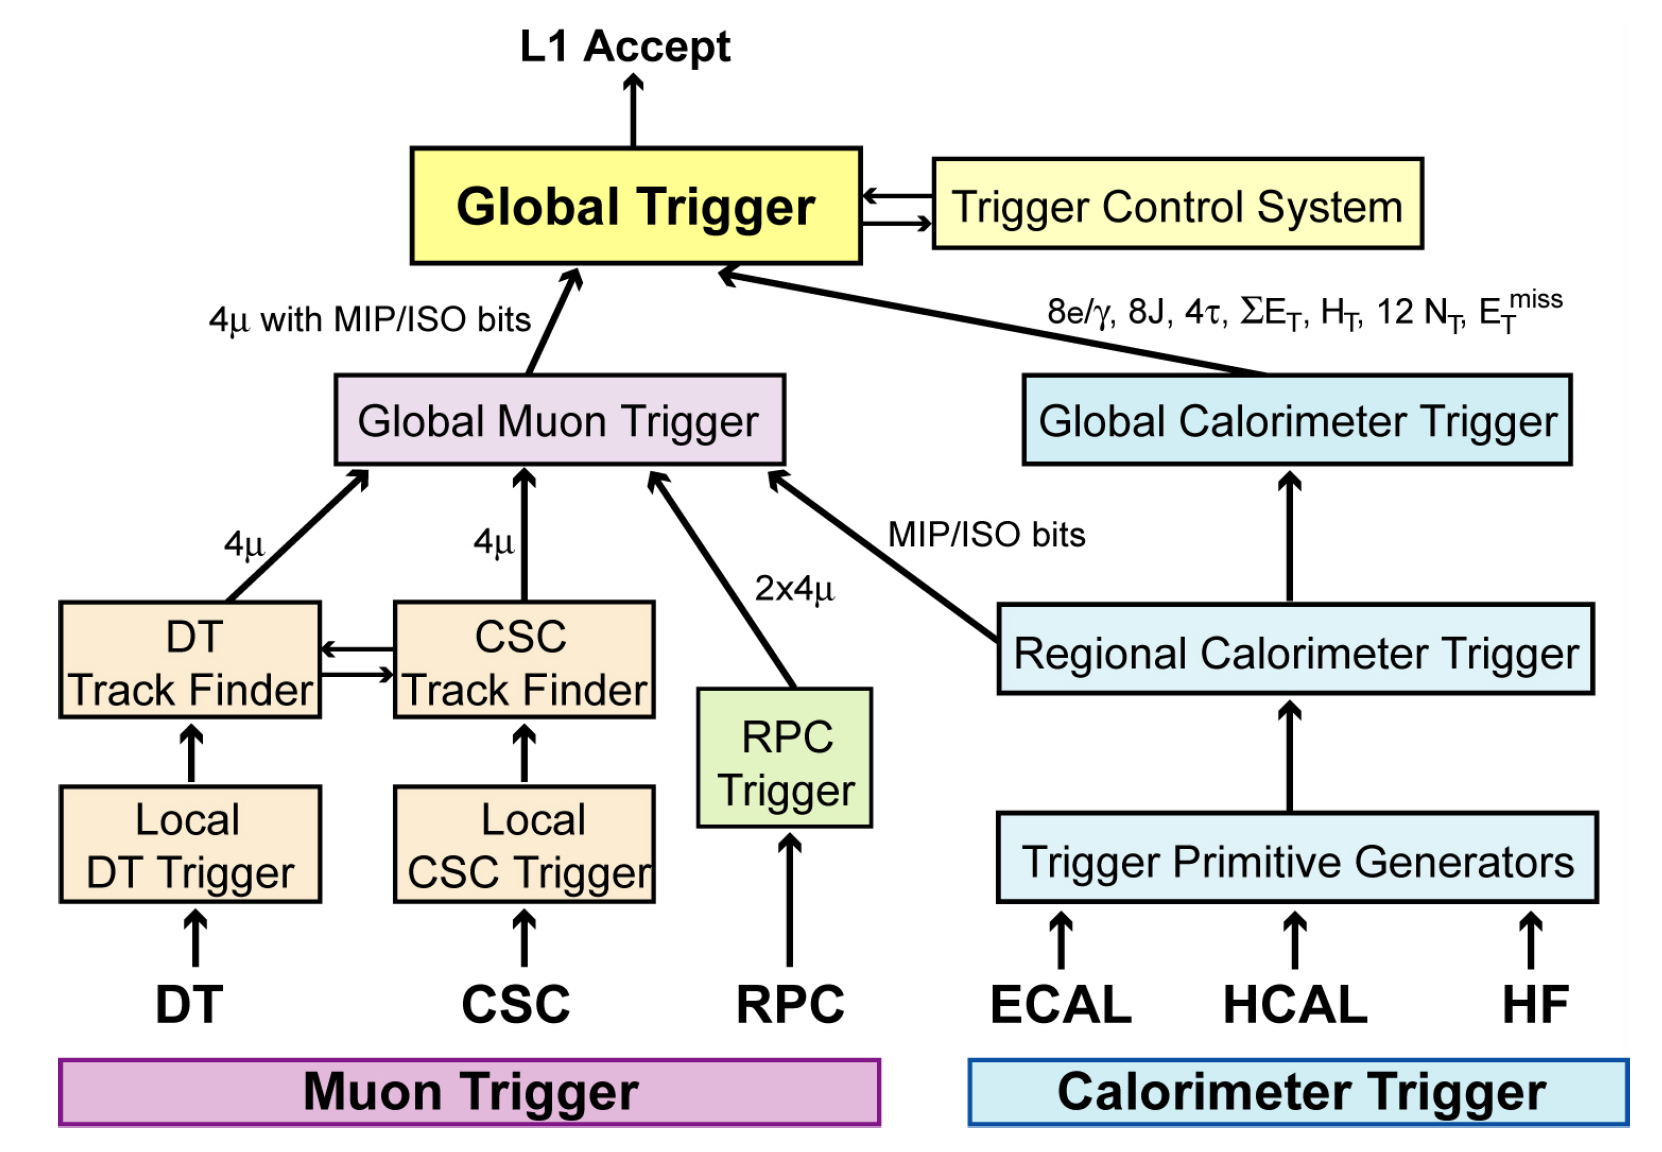
\includegraphics[width=0.70\textwidth]{figures/L1_trigger.png}
	\caption{A flowchart showing how the global, regional, and local components of the L1 trigger system operate to produce an L1A~\cite{Chatrchyan:2008aa}.}
	\label{fig:L1_trigger}
\end{figure}


The HLT consists of a processor farm running the full CMS online event reconstruction software, which can be continuously updated to meet experimental needs. A sophisticated data acquisition (DAQ) system works with the trigger system to collect and analyze the event information from each LHC bunch crossing. At designed luminosity, the LHC delivers about 1~MB/event of zero-suppressed data containing the full CMS detector information. The DAQ is designed to sustain a maximum input rate of 100~kHz and a data flow rate of approximately 100~GB/s. The HLT reduces the event rate to about 1~kHz. Events are uniquely specified by their run number, luminosity section of the LHC fill, and event number, all specific to the CMS DAQ system.



